\documentclass[12pt]{IEEEtran}

\usepackage[utf8]{inputenc}
\usepackage{amsfonts,amsmath,amsthm,amssymb,dsfont,mathtools}
\usepackage{geometry}
\usepackage{graphicx}
\usepackage{hyperref}
\usepackage{enumitem}
\usepackage{bookmark}
\usepackage{cite}
\usepackage{algorithm}
\usepackage{algpseudocode}
\usepackage{braket}
\usepackage{tikz}
\usetikzlibrary{shapes,arrows.meta,positioning}
\newcommand{\ketbra}[2]{\mathinner{|{#1}\rangle \langle{#2}|}}
\newcommand*\xor{\oplus}
\bibdata{references}
\usetikzlibrary{quantikz2}

\geometry{a4paper, margin=1in}


\title{\Large{Response to Ramesh \& Vinay, (2003)\\ \small{\textit{String Matching in \(\tilde{O}(\sqrt{n} + \sqrt{m})\) Quantum Time}} }}

\author{%
\normalsize{Matthew Evans, Ariz Siddiqui, Nathan Puskuri}
}
\date{\today}
\begin{document}

\maketitle

\section{Overview}
\textit{Ramesh \& Vinay, (2003)}\cite{RameshH2003SmiO} addresses the problem of efficiently determining whether a smaller string (pattern) appears within a larger one (text). Traditional solutions to this problem on classical computers take time roughly proportional to the total length of both the pattern and the text. The authors propose a quantum algorithm that determines the existence of a match with probability better than \(\frac{1}{2}\). While constrained in scope, their approach demonstrates how quantum computing methods, particularly quantum search techniques, can potentially achieve faster-than-classical performance for specific string matching scenarios.

We will first cover the concepts and dependencies to which the authors appeal, and then explain how these pieces fit together to support the authors' claims.

\section{Preliminaries}
\subsection{Grover's Algorithm}
Grover's algorithm \cite{grover1996fastquantummechanicalalgorithm} addresses the problem of locating one of \(t\) marked items in an unsorted database of \(N\) entries with a quadratic speedup over classical search. The procedure comprises the following steps:
\begin{enumerate}
    \item Initialize a superposition over all \(N\) basis states.
    \item Apply the oracle \(O_f\) to flip the phase of the marked state.
    \item Perform the diffusion operator to reflect amplitudes about their average.
    \item Repeat the oracle and diffusion operations approximately \(\frac{\pi}{4}\sqrt{N}\) times.
    \item Measure the register to obtain a marked element with high probability.
\end{enumerate}
Running in \(O(\sqrt{N})\) time, Grover's algorithm provides the core quantum search subroutine underpinning the \(\widetilde{O}(\sqrt{n}+\sqrt{m})\) string-matching algorithm.

\subsection{Tight Bounds on Grover's (BBHT96)}
\cite[Boyer, Brassard, Høyer, and Tapp]{Boyer_1998} show that even when the exact number of target items \(t\) in an unsorted database of size \(N\) is unknown, one can still locate a marked element in \(O(\sqrt(N/t))\) oracle calls with constant success probability. 
Their procedure adaptively adjusts the number of Grover iterations to achieve the same quadratic speedup without prior knowledge of \(t\). In our string-matching algorithm, this result is crucial: when searching a text block of length \(m/2\) for any matching alignment, we do not know in advance how many alignments will succeed, so we invoke BBHT96's method to retain the overall \(\widetilde{O}(\sqrt{n} + \sqrt{m})\) runtime bound.

\subsection{Deterministic Sampling (VI)}
Deterministic sampling, introduced by \cite[Vishkin]{10.1145/100216.100235} is a procedure for reducing the number of expensive pattern-matching checks on an aperiodic pattern \(p\) of length \(m\).  When matching \(p\) against a text block of length \(m/2\), there are \(m/2\) possible alignments.  Deterministic sampling picks \(O(\log m)\) indices in the pattern such that at most one alignment can match at all of these sample positions.  The procedure is:

\begin{enumerate}
    \item Form \(m/2\) ``copies'' of the pattern, each shifted by one position.
    \item Identify a column (i.e. pattern index) where at least two copies have different symbols.
    \item Choose one of the observed symbols as the sample value and discard all copies that do not match it.
    \item Repeat the previous two steps \(O(\log m)\) times until only one copy remains.
    \item Collect the chosen columns; these indices constitute the deterministic sample \(S\).
\end{enumerate}

Because only the single surviving alignment must undergo a full (quantum) check of cost \(\tilde O(\sqrt m)\), deterministic sampling reduces the number of such expensive checks per text block from \(m\) to \(1\).  This reduction is crucial to achieving the overall \(\widetilde{O}(\sqrt n + \sqrt m)\) runtime of the quantum string-matching algorithm.

\subsection{Minimum Finding Oracle}
The minimum-finding oracle given by \cite[Durr \& Høyer]{durr1999quantumalgorithmfindingminimum} locates the index of the smallest element in an unsorted database of size \(n\) in \(O(\sqrt{n})\) time using a comparison oracle. Beginning from a random index \(k\), it invokes Grover's algorithm to find any index \(i\) such that \(\text{database}[i]<\text{database}[k]\). If one is found, \(k\) is updated to \(i\) and the search repeats; if not, \(k\) is the minimum. This primitive underlies every ``pick the smallest (or leftmost) index satisfying some condition'' step in the paper. It is used to build the deterministic sample for aperiodic patterns—repeatedly halving the \(m/2\) candidate alignments in \(\widetilde{O}(\sqrt{m}\log m)\) time—and is invoked a second time to pinpoint the earliest text block containing the match, thereby preserving the overall \(\widetilde{O}(\sqrt{n}+\sqrt{m})\) runtime bound.

\begin{figure*}[!t]
    \centering
    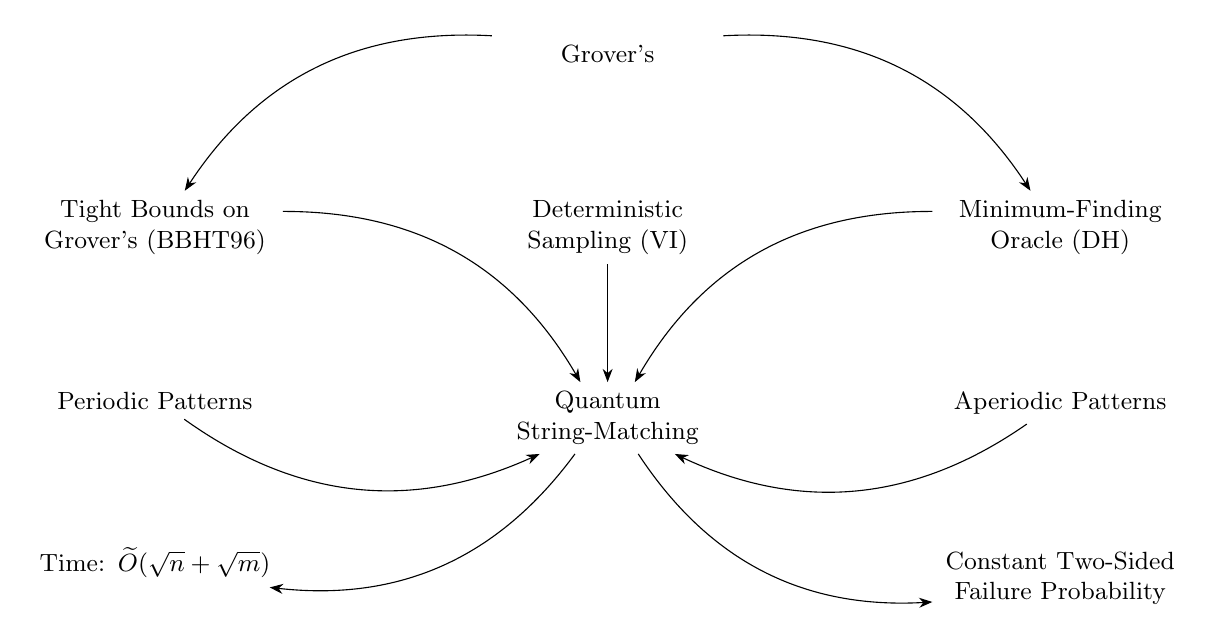
\begin{tikzpicture}[
        >={Stealth[]},
        every node/.style={font=\small, text width=3cm, align=center},
        node distance=1.5cm and 2.5cm
        ]
        % Nodes with plain text only
        \node (proposed)  {Quantum String-Matching};
        \node (vi) [above=of proposed] {Deterministic Sampling (VI)};
        \node (grover) [above=of vi] {Grover's};
        \node (bbht) [below left=of grover] {Tight Bounds on Grover's (BBHT96)};
        \node (dh) [below right=of grover]  {Minimum-Finding Oracle (DH)};
        \node (aper) [below=of dh] {Aperiodic Patterns};
        \node (periodic) [below=of bbht] {Periodic Patterns};
        \node (time) [below=of periodic] {Time: $\widetilde{O}(\sqrt{n}+\sqrt{m})$};
        \node (prob) [below=of aper]{Constant Two-Sided Failure Probability};

        % Curvy edges
        \draw[->, bend right]  (grover)   to (bbht);
        \draw[->, bend left] (grover)   to (dh);
        \draw[->, bend left]  (bbht)     to (proposed);
        \draw[->, bend right] (dh)       to (proposed);
        \draw[->]  (vi)       to (proposed);
        \draw[->, bend left]  (aper)     to (proposed);
        \draw[->, bend right] (periodic) to (proposed);
        \draw[->, bend left]  (proposed) to (time);
        \draw[->, bend right] (proposed) to (prob);
    \end{tikzpicture}
    \caption{Conceptual dependencies in the $\widetilde{O}(\sqrt{n}+\sqrt{m})$ quantum string-matching algorithm.}
    \label{fig:quantum-string-matching}
\end{figure*}

\section{Quantum String Matching}
\subsection{The Algorithm}
\begin{enumerate}
    \item \textbf{Deterministic-Sampling Preprocessing.}
          \begin{itemize}
              \item Run Vishkin's deterministic-sampling on \(p\) of length \(m\) to obtain an \(O(\log m)\)-sized sample set \(S\).
              \item Cost: \(\widetilde O(\sqrt{m}\,\log^2 m)\).
          \end{itemize}
    \item \textbf{Partition the text.}
          \begin{itemize}
              \item Divide the text \(t\) into
                    \[
                        B \;=\; \left\lceil \frac{2(n - m + 1)}{m} \right\rceil
                    \]
                    blocks, each of size \(\approx m/2\).
          \end{itemize}
    \item \textbf{Quantum search for a ``hit'' block.}
          \begin{itemize}
              \item Define oracle \(h(i)\): tests if block \(i\) has at least one alignment matching on all positions in \(S\) in \(\widetilde O(\sqrt{m}\,\log m)\) time.
              \item Use Grover search over \(i=1,\dots,B\) with oracle \(h\); time \(\widetilde O(\sqrt{n}\,\log m)\). If none found, conclude ``no occurrence.''
          \end{itemize}
    \item \textbf{Locate surviving alignment in block.}
          \begin{itemize}
              \item Define oracle \(k(i^*,j)\): checks alignment at shift \(j\) in block \(i^*\) on sample \(S\) in \(O(\log m)\) time.
              \item Use Grover search over \(j=0,\dots,\lfloor m/2\rfloor\) with oracle \(k\); time \(\widetilde O(\sqrt{m}\,\log m)\). If none survives, conclude ``no occurrence.''
          \end{itemize}
    \item \textbf{Full quantum verification.}
          \begin{itemize}
              \item Run Grover search over \(\ell=1,\dots,m\) with oracle ``\(t[i^*+j^*+\ell]\neq p[\ell]\)'' to find any mismatch; time \(\widetilde O(\sqrt{m})\).
              \item If no mismatch is found, report occurrence at \(i^*+j^*\); otherwise, conclude ``no occurrence.''
              \item Cost: \(O(\sqrt{m})\)
          \end{itemize}
\end{enumerate}
Overall time: \(\widetilde O(\sqrt{m}\,\log^2 m) + O(1) + O(\sqrt{n} \log m) + O(\sqrt{m} \log m) + O(\sqrt{m}) = \widetilde{O}(\sqrt{n} + \sqrt{m})\)

\subsection{Concerning Periodicity}
% discuss periodic vs. aperiodic patterns

\subsection{Constant Two-Sided Failure Probability}
The h(i) oracle which detects if a block contains a match succeeds with probability 3/4 and the following k(i,j) block can identify the correct starting position in the block with probability 3/4.
The combined probability of success will be $frac{9}{16}$. The failure probability will be $frac{7}{16}$. There are two possible errors here. The oracle h(i) might fail to flag a block that contains a match or 
the oracles h(i) and k(i,j) detect a match in a block that does not have one. So we can either get a false negative or false positive. The algorithm has a fixed chance of error which is 1-9/16=7/16. 
We can reduce this error by repeating the process multiple times so the failure probability goes down to \(\frac{7}{16}^t\). 
% discuss the importance of the constant two-sided failure probability as mentioned in the paper
\subsection{Achieving \texorpdfstring{$\tilde{O}(\sqrt{n} + \sqrt{m})$}{O(sqrt(n)+sqrt(m))}}

% bring everything together. Give a run-through of the entire algorithm, putting all the pieces together. 

\bibliographystyle{plain}
\bibliography{references}
\end{document}